\documentclass[review]{elsarticle}

\usepackage{lineno,hyperref}
\modulolinenumbers[5]

\usepackage[top=2.54cm, bottom=2.54cm, left=2.54cm, right=2.54cm]{geometry}
\usepackage{amsmath}
\usepackage{graphicx}
\usepackage{subfig}
\renewcommand{\thesubfigure}{\Alph{subfigure}}% uppercase subfloat numbering
\graphicspath{{../figures/}}
\usepackage[]{color}
\newcommand\hl[1]{{\textcolor{blue}{#1}}}

% some new commands to make non-italic ds in dx etc.
\newcommand{\dd}{\ensuremath{\mathrm{d}}}
\newcommand{\dbyd}[2]{\ensuremath{\frac{\dd #1}{\dd #2}}}
\newcommand{\partialdbyd}[2]{\ensuremath{\frac{\partial #1}{\partial #2}}}
\newcommand{\functionaldbyd}[2]{\ensuremath{\frac{\updelta #1}{\updelta #2}}}

\journal{Journal of Theoretical Biology}

%%%%%%%%%%%%%%%%%%%%%%%
%% Elsevier bibliography styles
%%%%%%%%%%%%%%%%%%%%%%%
%% To change the style, put a % in front of the second line of the current style and
%% remove the % from the second line of the style you would like to use.
%%%%%%%%%%%%%%%%%%%%%%%

%% Numbered
%\bibliographystyle{model1-num-names}

%% Numbered without titles
%\bibliographystyle{model1a-num-names}

%% Harvard
%\bibliographystyle{model2-names.bst}\biboptions{authoryear}

%% `Elsevier LaTeX' style
\bibliographystyle{elsarticle-num}
%%%%%%%%%%%%%%%%%%%%%%%

\begin{document}

\begin{frontmatter}

\title{Neural crest migration with continuous cell states}

%% Group authors per affiliation:
\author{Linus J. Schumacher\fnref{myfootnote}}
\address{MCR Centre for Regenerative Medicine, University of Edinburgh}
\ead{Linus.Schumacher@ed.ac.uk}


\begin{abstract}
Models of cranial neural crest cell migration in cell-induced (or self-generated) gradients have included a division of labour into leader and follower migratory states, which undergo chemotaxis and contact guidance, respectively. Despite validated utility of these models through experimental perturbation of migration in the chick embryo and gene expression analysis showing relevant heterogeneity at the single cell level, an often raised question has been whether the discrete cell states are necessary, or if a continuum of cell behaviours offers a functionally equivalent description. Here we argue that this picture is supported by recent single-cell transcriptome data. Motivated by this, we implement two versions of a continuous state model: (1) signal choice and (2) signal combination. We find that migration is more persistent than in the discrete state model and than in experimental observations. We further show that the signal combination model, but not the signal choice model, can be successfully adjusted to experimentally plausible regimes by reducing the chemoattractant consumption parameter. Thus we show an equivalently plausible, experimentally motivated, model of neural crest cell migration.
\end{abstract}

\begin{keyword}
collective behaviour \sep cell migration \sep developmental biology
\MSC[2010] 92C15
\end{keyword}

\end{frontmatter}

\linenumbers

\section{Introduction}
Neural crest cell migration is a popular example of collective cell behaviour in development. Neural crest cells migrate over long distances in the vertebrate embryo and contribute to a variety of tissue types. Understanding their migration is important to identify the causes for birth defects, and they also provide a model system to study the invasive migration of cancer cells, especially the neural crest derived melanoma \cite{Kulesa2006,Bailey2012,McLennan2017}. Mechanisms of neural crest cell migration have been studied in a variety of model organisms, and multiple groups have approached the problem with mathematical modelling \cite{Simpson2007,Landman2011,Carmona-Fontaine2011,Wynn2012,Wynn2013,McLennan2012,McLennan2015,Mort2016,Zhang2018,Merchant2018}. %% longer?

Previous work has shown that chick cranial neural crest cell migration can be described with discrete leader-follower states that alternatively undergo chemotaxis or contact-guidance \cite{McLennan2012,McLennan2015}, and switch between the two on a non-zero timescale based on VEGF signals \cite{McLennan2015b}. The utility of this model has been validated in a number of ways, such as using the model to predict the outcome of tissue transplantation experiments \cite{McLennan2012,McLennan2015,McLennan2015b}, and gene expression analysis \cite{McLennan2015,McLennan2015b}, including recent single-cell RNAseq \cite{Morrison2017}. While earlier studies identified key differences between neural crest sub-groups for selected genes, the advent of single-cell whole transcriptome analysis provides an opportunity to investigate the heterogeneity of the neural crest subpopulation in a less biased way. %% more specific?

What has hitherto not been investigated is whether leader-follower cell states need be discrete, or could lie on a continuum. This question is relevant in light of ongoing debate in the literature about whether mechanisms of neural crest cell migration are common or distinct in different model organisms \cite{Schumacher2016a,Richardson2016,Genuth2018}. Here theoretical biology can provide a useful argument, due to the difficulty of inferring heterogeneity from cell tracking data alone \cite{Schumacher2017}. From a molecular perspective, such questions about cellular identity are now just coming within reach of experimental measurement \cite{Wagner2016}, making this a highly timely topic of enquiry. %% more specific?

Here we address whether chick cranial neural crest cell migration can be described with continuous cell states equally well as existing models and with experimentally plausible outcomes. We first revisit recently published single-cell transcriptome data \cite{Morrison2017} to show that a continuum of cell states is not ruled out by the data. We then modify previous models \cite{McLennan2015,McLennan2015b} to assess what effect a continuum of cell guidance behaviours has on the collective migration, providing two alternative implementations of choosing between chemotaxis and contact guidance, or combining information from both signals. We find that the naive implementation of continuous states achieves unrealistic migration outcomes with cells migrating too far, and explore how the models can be modified to remedy this without sacrificing total cell number. The signal combination model can be successfully adjusted by reducing the chemoattractant consumption rate, thus providing a reasonable alternative (or equivalent) to the model of discrete leader and follower states. We finish by discussing model robustness and plausible alternative modifications. % rephrase?

\section{Results}
\subsection{Analysis of single-cell transcriptome supports continuum of cell states}
Previous models have shown that migration in a cell-induced gradient can be more successful with fewer cells in a leader state, suggesting heterogeneity of cell states at the scale of a few or tens of cells, which has been confirmed with RT-qPCR \cite{McLennan2015}. Recently published single-cell RNAseq data \cite{Morrison2017} is a less biased way to measure the heterogeneity of gene expression in a cell population, as it measures the whole transcriptome instead of selected genes. The published analysis of this dataset focussed on the identification of gene-signatures based on the pairwise differential expression between groups, such as cells from trailing, lead, and front portions of the migratory stream \cite{Morrison2017}. An alternative approach is to explore the data with the question of whether cell states may be discrete or continuous.

Analysis of single-cell transcriptomes is challenging because many (thousands) genes are sampled and cell numbers can be low (hundreds), particularly when they have to be individually dissected. Here we utilize an approach from random matrix theory that discerns how many principal components of a data-set can be expected to result from non-random correlations given the size of the data set. This approach has previously been used for single-cell gene expression analysis\cite{Klein2015a}, and recently published as a software tool \cite{Aparicio2018} to separate out the signal from the noise in the variation of gene expression between cells. In the neural crest data set \cite{Morrison2017}, we focus on in vivo cells from chick embryo stages HH13\&15, were we have cells from trailing, lead, and invasive front portions of the stream. We find that 59 dimensions are non-trivial (Fig.~\ref{figMP}). The resulting 59-dimensional dataset is mapped to two dimensions using a force-based embedding approach \cite{Weinreb2018}. Labelling cells according to where in the stream they were sampled from, this exploratory visualisation of the population structure broadly maintains the order of spatial positions in the stream of trail, lead, front (Fig.~\ref{figscRNAseq}). There is further structure visible in the data, with the possible existence of subgroups comprising all three sample categories, which we don't investigate further here. Overall, there is mixing and overlap between the sample categories, but with a discernible ordering, which supports the view that cell states may be continuous.

\begin{figure}
    \centering
    {\includegraphics[scale=0.45]{NCstates.pdf}}
    \caption{Visualisation of a continuum of neural crest cell states \hl{based on gene expression}. Single-cell RNAseq data (published in \cite{Morrison2017}) from chick cranial neural crest (Hamburger-Hamilton stages 13 and 15, 310 cells in total) taken from distinct locations in the migratory stream (trail: dark green, lead: light green, invasive front: pale yellow) were projected onto two dimensions for visualisation using a force-based embedding method \cite{Weinreb2018}. Only the top 59 principal components (out of 14299 genes measured, 12909 after preprocessing) were retained prior to embedding, based on random-matrix analysis \cite{Aparicio2018} (Fig.~\ref{figMP}). \hl{Note that while the rotation of this embedding is arbitrary, the ordering of cells in gene expression space is reminiscent of the structure of the migratory stream (with invasive front to trailing cells here oriented right to left), while also supporting a continuum of cell states.}\label{figscRNAseq}}
\end{figure}

\subsection{Model of neural crest cell migration}
Motivated by our exploratory analysis of single-cell RNAseq data, we wanted to investigate what effect a continuum of leader and follower migratory behaviours would have on the collective migration of neural crest cells. We built upon the existing model developed by the author and others \cite{McLennan2012,McLennan2015,McLennan2015b}, \hl{which we briefly describe in the following sections \ref{methodsRDE} and \ref{methodsABM} before explaining the new extensions to it in sections \ref{methodsSignalChoice} and \ref{methodsSignalCombination}}.

\subsubsection{Cell-induced gradient\label{methodsRDE}}
The model is a hybrid model with agent-based cell movement and a reaction-diffusion equation for the chemoattractant \eqref{RDE}, solved on a growing domain, with the cells acting as sink-terms, resulting in a cell-induced\cite{Kulesa2010a}, or self-generated gradient in the otherwise uniform chemoattractant \hl{(as also studied in other systems \cite{Streichan2011,Muinonen-Martin2014,Tweedy2016})}. \hl{The reaction-diffusion equation is of the form}
      \begin{equation}
        %\begin{split}
       \partialdbyd{c}{t} = D\nabla^2{c} - \lambda c\sum_{i=1}^{N(t)} \delta(\mathbf{x} - \mathbf{x}_i)+ \chi c(1 - c),
       %\end{split}
      \end{equation}

\hl{where $c$ is the chemoattractant concentration, $\lambda$ the internalisation rate by cells, $\mathbf{x}_i$ ths position of the $i$th cell, and $\xi$ the background production. For details of numerical implementation with tissue-growth see \eqref{RDE}. The initial conditions are spatially uniform chemoattractant, and the boundary conditions are no-flux. The two-dimensional domain is rectangular with growth in the x-drection, such that $(x,y) \in [0, L_x(t)]\times[0, L_y]$. Domain growth is prescribed by a logistic equation fitted to experimental measurements of tissue growth, see \eqref{domaingrowth}}.

\subsubsection{Cell movement\label{methodsABM}}
Cells enter the domain on one side, obeying volume exclusion, and sample discrete number of directions (representing filopodia) to look for favourable chemoattractant gradients or contact guidance, depending on whether they are in a leader or follower state. \hl{ For availability of the code, see Section \ref{modelcode}.} Cells can switch between these discrete states on a non-zero timescale \cite{McLennan2015b}, which is controlled by the exposure the chemoattractant gradient signal over time. \hl{This ``Integrate-and-Switch'' mechanism {\cite{McLennan2015b}} was introduced to incorporate the experimentally observed plasticity of cell states (see Section \ref{IntegrateAndSwitch} for details). However, this switch was not related to the magnitude of the gradient signal, and further raised the question whether a simplified model, without signal integration over time, would suffice.} Further modifications of this model included an inhibitory zone that can slow down cells and hence improve stream cohesion \cite{McLennan2017}, but we have not used this here. Previous versions of the model have implemented no-flux boundary conditions for the cells at the edge of the migratory domain. Here we instead adopt reflective boundary conditions that prompt cells to move away from the boundary, to more accurately represent the inhibitory zones \cite{Kulesa2010,Szabo2016a} that are thought to shape or confine the stream of cells. The change in boundary condition mainly changes the stream morphology (cells don't stay very close to the boundary), but do not effect the overall migration profiles.

%% add separate methods section elsewhere or sub-section here, and make sure to refer to SI

\subsubsection{Signal choice model\label{methodsSignalChoice}}
One alternative to discrete cell states that are restricted to make use of either chemotaxis or contact guidance (Fig.~\ref{figNaiveModel}A), is that each cell can choose between these two signals (Fig.~\ref{figNaiveModel}B). This model reflects the hypothesis that cells can sense both signals, but only act on one or the other at a given time. This is implemented by a stochastic choice between the two signals, where the probability is given by the \hl{cell's perceived chemoattractant gradient}. For simplicity, we have here chosen a linear relationship $P_{ch} = \Delta c$, where $\Delta c$ is the \hl{difference in chemoattractant concentration} measured between the cell body and its filopodial tip. This quantity is bounded between 0 and 1, as the chemoattractant concentration in our model is set in arbitrary units between 0 and 1, \hl{effectively normalising with respect to the uniform starting concentration}. The contact guidance signal is thus chosen with a probability of $P_{cg} = 1 - \Delta c$. Thus a cell's direction of movement, $\vec{\theta}$, is given by
\begin{equation} \label{eqnChoice}
     \vec{\theta} = 
         \begin{cases}
         \vec{\theta}_{ch}, & P_{ch} = \Delta c \\
        \vec{\theta}_{cg}, & 1 - P_{ch}
        \end{cases}
\end{equation}
where $\vec{\theta}_{ch}$ is the direction of the (sampled) chemoattractant gradient, and $\vec{\theta}_{cg}$ is the direction prescribed by contact guidance.
	\hl{The signal choice model differs from the "Integrate-and-Switch" model \cite{McLennan2015b} in that there is no signal integration over time. Instead of switching between discrete states, all cells are in the same state and choose their instantaneous actions. The probability used here is proportional to the chemoattractant difference, and this could be easily extended to non-linear relationships or other signals, such as co-attraction \cite{Carmona-Fontaine2011,Merchant2018}.}

\subsubsection{Signal combination model\label{methodsSignalCombination}}
A second possibility for continuous states is that each cell combined the directional information from chemotaxis and contact guidance (Fig.~\ref{figNaiveModel}C). This reflects the hypothesis that both signals generate a motile force in the cell's cytoskeletal machinery, and the cell moves in the resulting overall direction. We implement this by setting a cell's direction of movement as a weighted sum of the directions from contact guidance and chemotaxis, with the weighting determined by the strength of the chemoattractant gradient. For simplicity we have again chosen a linear weight, such that the overall direction is given by 
\begin{equation} \label{eqnCombination}
	\vec{\theta} = \Delta c\ \vec{\theta}_{ch} + (1 - \Delta c)\vec{\theta}_{cg},
\end{equation}
with the individual directions as above, \hl{and $\Delta c$ again being the difference in chemoattractant concentration measured between cell body and  filopodial tip}.

\subsection{Continuous states migrate further than discrete states}
To compare the original model with its two alternatives, we simulate migration for 18h and visualise the result as a histogram of number of cells vs distance migrated \hl{(defined as the maximum of the $x$-coordinates of all cells)}. Both the signal choice and signal combination models migrate further than the discrete state model (Fig.~\ref{figFurtherModel}D), and further than is typically observed experimentally. This can be interpreted as the cells have more directional information to act on and hence being able to migrate in a more directed manner towards the target zone at the end of the migratory route. We further observed that in this implementation of the continuous state model, cells stay attached to each other longer (Fig.~\ref{figFurtherModel}E), whereas previously leaders would not engage in contact guidance at all, and thus cells would detach when switching from the follower to the leader state. In the continuous state model, cells can instead stay attached to their nearby neighbours throughout migration, even if primarily undergoing chemotaxis. We thus considered two avenues to refine this initial implementation, by either breaking long-term cell-cell contact or affecting the gradient sensing. % mention/show stream break-up?
% reference for filopidal-cell contact times? (on the order of hrs)
\begin{figure}
    \centering
    \subfloat[]{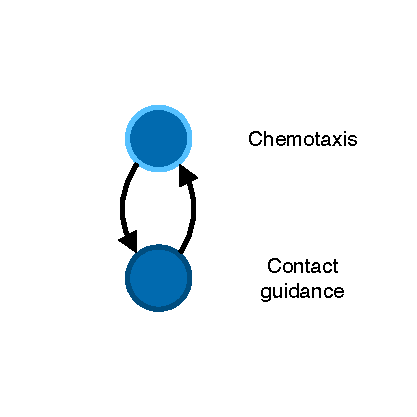
\includegraphics[]{modelSchematicControl}}
    \subfloat[]{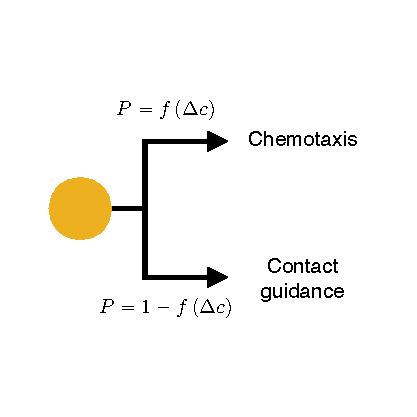
\includegraphics[]{modelSchematicChoice}}
    \subfloat[]{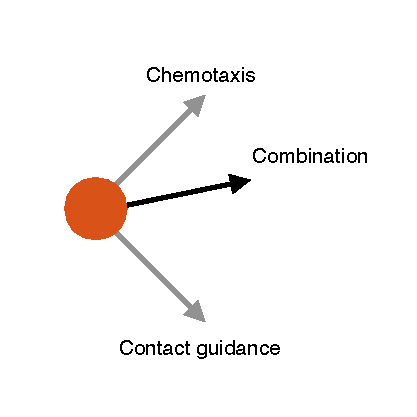
\includegraphics[]{modelSchematicCombination}}\\
    \subfloat[]{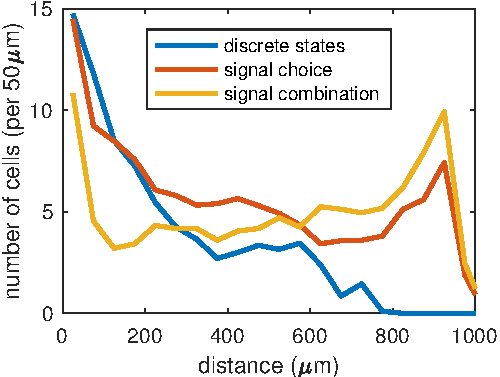
\includegraphics[]{Fig2_contStates_combination_sensAcc_10}}
    \subfloat[]{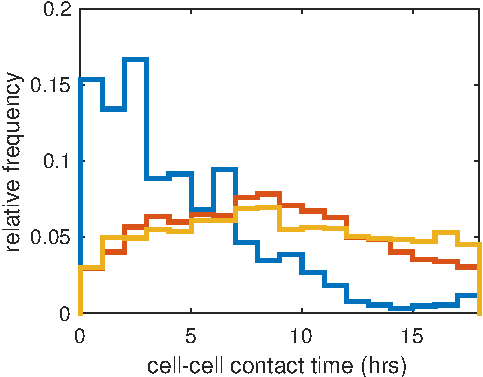
\includegraphics[]{Fig2B_contStates_combination_sensAcc_10}}
    \caption{Comparison of collective cell migration models with discrete and continuous states. (A) In the previously published model \cite{McLennan2015b}, cells switch between migratory states based on the presence of a chemotactic signal and at a non-zero timescale. (B) In the signal choice model, cells choose between chemotaxis and contact guidance for their direction of movement, with a probability related to the strength of the chemoattractant gradient. In results shown here, we have used $P_\mathrm{ch}=\Delta c$ for chemotaxis and $P_\mathrm{cg}=1 - \Delta c$ for contact guidance,  \hl{where $\Delta c$ is the difference in chemoattractant concentration measured between cell and filopodium}. (C) In the signal combination model, cells combine the directional information from both chemotaxis and contact guidance, with a weighting depending on the strength of the gradient signal. Here we have used a linear weight of $\Delta c$. (D) Migration profiles of the three models after 18h of migration. (E) Durations of cell-cell contacts during migration for the three models. \hl{Contact duration is calculated from the number of consecutive time-steps that a cell is contacting another with a filopodium.} Line colours as in (D). (C,D) Data shown are averages over 20 simulations for the discrete state model, and 40 simulations for each of the signal choice and signal combination models. \label{figNaiveModel}}
\end{figure}

\subsection{Reducing contact guidance persistence reduces cell number and distance migrated}
To prevent the unrealistically long filopodia-cell contact times observed in the continuous state models (Fig.~\ref{figNaiveModel}E), we allowed a cell's filopodia to detach stochastically from the cell it is in contact with, with probability $P_d$ at every time-step. We then varied the detachment probability to assess whether a reduction in the distance migrated could be achieved without a large loss in the total cell number, as this represents the experimentally plausible scenario in unperturbed in vivo migration. Simulation results show that increasing the detachment probability in either the signal choice or signal combination models (Fig.~\ref{figFurtherModel}A) does decrease the distance migrated, but also rapidly decreases total cell number. Hence, reducing the persistence of contact guidance is insufficient to make the continuous state models biologically plausible.

\begin{figure}
\centering
\subfloat[]{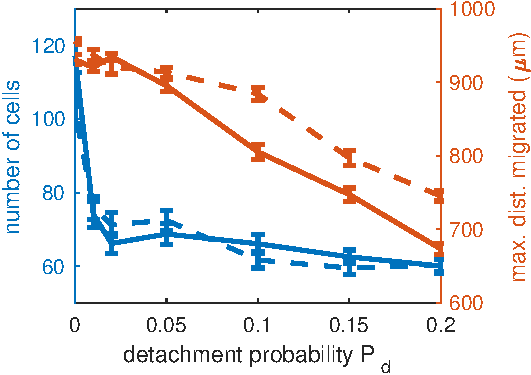
\includegraphics[]{Fig3_contStates_Psa_sensAcc_10}}\
\subfloat[]{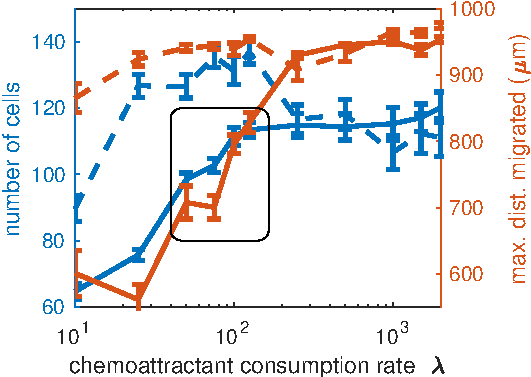
\includegraphics[]{Fig3_contStates_eat_sensAcc_10}}
\caption{Modifications to the continuous-state models can achieve experimentally realistic results. (A) Introducing a detachment probability, $P_d$, for the filopodial contacts used for contact guidance decreases the maximum distance migrated \hl{(defined as the maximum of the $x$-coordinates of all cells)}, but only at the cost of \hl{decreasing the} total cell number for both the signal choice model (dashed lines) and the signal combination model (solid lines). (B) Reducing the chemoattractant consumption rate, $\lambda$, to the range of 40-150 (arbitrary units per hour) achieves realistic maximum distances migrated, with only a moderate reduction in cell number (highlighted by the black rectangle) for the signal combination model (solid lines), but not the signal choice model (dashed lines). Data shown are averages over 40 simulations for each parameter value, error bars show standard error of the mean.\label{figFurtherModel}}
\end{figure}

\subsection{Shallower cell-induced gradients enable the signal combination model}
We reasoned that affecting the model parameters relating to the chemoattractant may make the cell migration in the continuous state models less directed. Reducing the chemoattractant consumption, $\lambda$, of the cells decreases the sink-term in the reaction-diffusion equation, and should hence create shallower local gradients in the chemoattractant. \hl{With lower chemoattractant consumption, the distance migrated decreases, as does the total cell number. For the signal combination model, there is an intermediate regime where the distance migrated is at experimentally observed values, but the total cell number is still high} (for the range $\lambda=40-150$, arbitrary units per hour) (Fig.~\ref{figFurtherModel}B). This was not the case for the signal choice model. The behaviour is otherwise robust for wide ranges of the experimentally less-constrained parameter values, chemoattractant diffusivity and background production (Fig.~\ref{figNaiveModelSweeps}A\&B), with the exception of very high chemoattractant diffusivity in the combination model, which showed low cell numbers. 
% cite Insall?

\section{Conclusions}
We have revisited the model of chick cranial neural crest migration to address the question whether leader/follower (chemotaxis/contact guidance) cell migratory states could be continuous rather than discrete (Fig.~\ref{figNaiveModel}A). This was motivated in part by debates in the field, and in part by the recent availability of transcriptome data at single cell resolution. We reanalysed published gene expression data and found that this can support a continuum of cell states (Fig.~\ref{figscRNAseq}). Starting from our previous cell migration model, we then implemented two versions of a continuous state model, in which cells either choose between directional signals (Fig.~\ref{figNaiveModel}B) or combine the directional information (Fig.~\ref{figNaiveModel}C). The initial implementations of these models, without any further modifications, showed more persistent migration than the discrete state model (Fig.~\ref{figNaiveModel}D), with the distance migrated overshooting experimentally observed values. By changing the chemoattractant consumption, a key parameter that determines the cell-induced/self-generated gradient, we \hl{were able to adjust} the signal combination model to achieve experimentally observed migration distances without an drastic reduction in total cell number.

%\paragraph{need other methods for dealing with various sources of noice in single cell data to decompose ``vectors of cellular identity'' \cite{Wagner2016}}

It is possible that other model modifications would have had a similar effect. We could have chosen a non-linear relationship for the weighting in combining chemotaxis and contact guidance. Further to this, one could refine the model by making the chemoattractant consumption proportional to a cells ``leaderness'', based on the experimental observation that VEGF receptor expression is higher in cells at the invasive front \cite{McLennan2015,Morrison2017}. Based on our assessment presented here, the stochastic choice model is less plausible than the combination model. The role of stochasticity has also been investigated in other aspects of neural crest migration, such as colonisation of the gut \cite{Binder2015,Smadbeck2015,Zhang2018} and pigmentation patterning \cite{Mort2016}, and one could further explore the role of noise in contact guidance, for example by adding angular noise to the directional signal sensed, which we would expect to reduce the persistence of migration. Extending the model to 3D could also reduce \hl{the} distance moved in the primary direction of migration, as more of the movement would be along the other two dimensions. \hl{A mathematically more challenging prospect for further work is to derive appropriate continuum equations, in which cells move in physical space as well as in cell state space.} We can readily conceive of other versions of a continuous state model that may be realistic presentations of the neural crest migration, our work shows at least one such example, and that continuous state models ought to be taken into account.

Our results point to avenues for further experimental quantification, which in turn would constrain the models. The comparison with experimental data in these models has been largely semi-quantitative due to the limitations in quantifying relevant statistics such as total cell number and distance migrated. Distance migrated is not absolutely quantified experimentally, due to embryo-to-embryo size variation, and a missing consensus on what to measure as a start-point. Further difficulties arise due to the incomplete labelling efficiency of electroporated fluorescent markers. The time over which cell-cell contacts mediating contact guidance persist has not been quantified across the whole migratory population \cite{Teddy2004}, yet \hl{the long-term contacts we observed} in the continuous state models seem unrealistic. % rephrase? reference electroporation efficiency? reference contact-time?

Alternatives to the chemotaxis and contact guidance paradigm have been put forward in related work. Contact-inhibition of locomotion has been studied as a mechanism enabling collective migration both in computational models and in \textsl{Xenopus} embryos \cite{Carmona-Fontaine2011}, but this has not been observed in chick cranial neural crest \cite{Genuth2018}. Another alternative to contact guidance would be pulling of followers by leader cells \cite{Yates2018}, and vice versa, which would improve overall stream cohesion. Preliminary simulations in which cells require sufficient neighbours to move show that this can also reduce migration (Fig.~\ref{figNaiveModelSweeps}C). \hl{This would be a purely contact-based mechanism distinct from theories of collective chemotaxis, in which cells communicate their chemoattractant measurements to arrive at a improved consensus \cite{Camley2016}. This form of collective chemotaxis has, to our knowledge has not been explored in neural crest cell migration.} To assess the robustness of mechanisms proposed here (and alternative models) beyond sensitivity analysis of individual parameters as done here, future work \hl{could adopt a parameter inference approach}, as has been done for other models of collective cell migration \cite{Ross2017}.

In conclusion, we have shown that a model of chick cranial neural crest migration can work with continuous cell states. This suggests our previous model with discrete states may be an approximation of continuous state models, and whether this makes the mechanism simpler or more complex depends on the perspective. We have provided a step towards unifying competing views in the literature \cite{Schumacher2016a}. A similar model-based approach to investigate discrete vs continuous states could be applied beyond neural crest cell migration, such as development of the lateral line \cite{Dona2013} and asymmetry in the brain \cite{Roussigne2018} in zebrafish, \textsl{Drosophila} border cells \cite{Inaki2012}, and in collective migration of organisms. \hl{This study has considered collective cell migration, but the question of whether cell states are best described as discrete or continuous arises in many other biological problems. Analogous modelling frameworks could help to investigate the effect of continuous cell states in stem cell quiescence \cite{Basak2018}, proliferation \cite{Macklin2017,Yates2017}, and differentiation \cite{Greulich2016,Stumpf2017}.} 

\section*{Acknowledgements} The author is supported through a Chancellor's Fellowship at the University of Edinburgh.%I would like to thank Franziska Matth\"aus for persistent suggestions. 
\section*{Appendix}
\renewcommand{\thefigure}{S\arabic{figure}}
\setcounter{figure}{0}
\renewcommand{\thesection}{S}

\begin{figure}
\centering
\subfloat[]{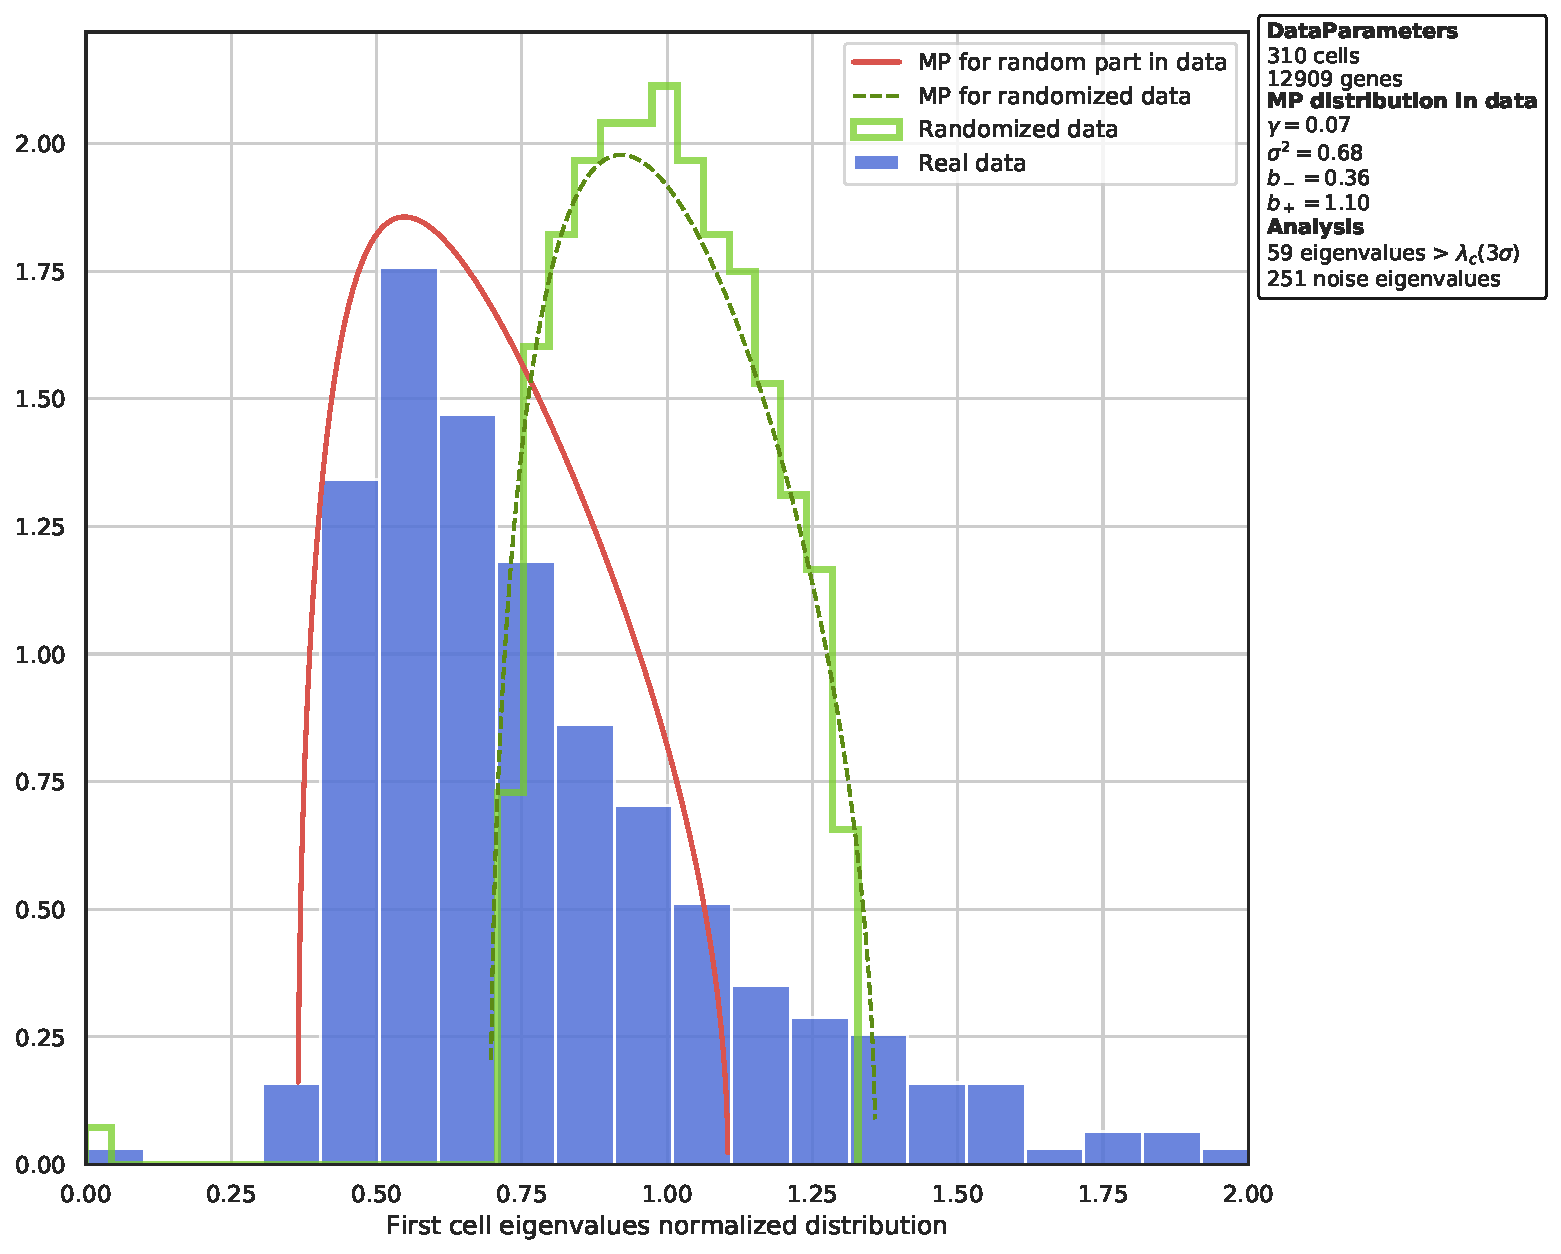
\includegraphics[scale=0.65]{mp_NC_HH1315}}
\caption{Distribution of eigenvalues of the cross-correlation matrix as calculated by the ``randomly'' software package \cite{Aparicio2018} for the single-cell RNAseq data from \cite{Morrison2017}. Bigger eigenvalues correspond to principal components that explain more variance of the data. Random matrix theory predicts that the eigenvalues of the cross-correlation matrix of a set of independent identically distributed random variables are distributed according to the Marchenko-Pastur law. Hence, a certain amount of correlation in a data-set is to be expected under the null model of independence, here shown in red, and only principal components with large enough eigenvalues are treated as signal (here, the top 59 eigenvalues). \label{figMP}}
\end{figure}

\begin{figure}
\centering
\subfloat[]{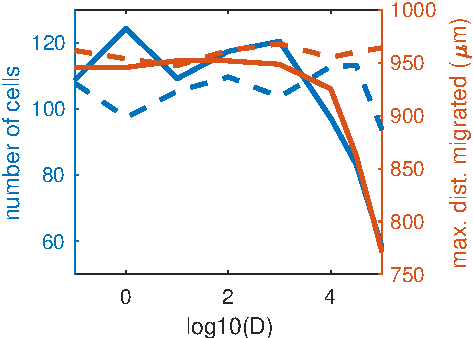
\includegraphics[]{FigS2_contStates_diffus_sensAcc_10}}\quad
\subfloat[]{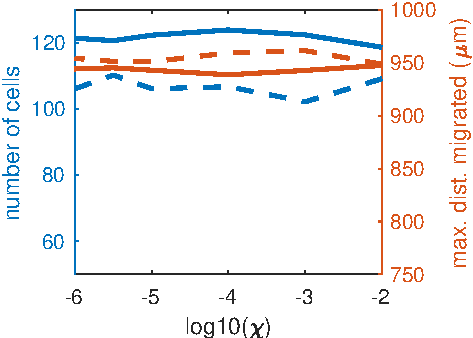
\includegraphics[]{FigS2_contStates_chi_sensAcc_10}}\\
\subfloat[]{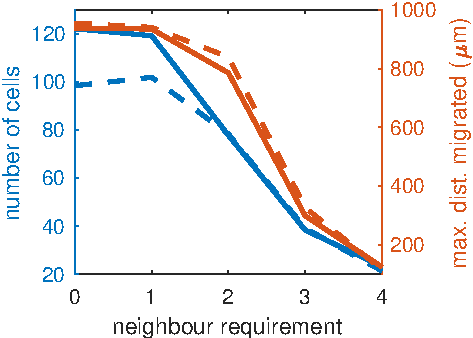
\includegraphics[]{FigS2_contStates_needNbrs_sensAcc_10}}
\caption{Further analysis of the continuous states model, showing total number of cells and maximum distance migrated after 18h of migration \hl{(defined as the maximum of the $x$-coordinates of all cells)}, varying (A) the chemoattractant diffusivity, D ($\mu m/h$), (B) the background chemoattractant production, $\chi$ (arbitrary units per hour), and (C)  introducing a neighbour requirement, such that cells only move in a directed manner if they have at least $n$ neighbours within filopodial reach. Data shown are averages over 40 repeated simulations for each parameter value.\label{figNaiveModelSweeps}}
\end{figure}

\begin{table}[htbp]
    		\caption{\bf Model parameters} Parameter values listed were used as a default, unless otherwise stated, e.g., in the parameter sweeps of Fig. \ref{figFurtherModel} \& \ref{figNaiveModelSweeps}. The chemoattractant concentration is implemented in relative units, such that the starting value $c_0=1$.\\
    
    	\centering
    		\begin{tabular}{llll} \label{parameters}
    			 & Description & Value & Reference \\
    			\hline            
                $n_\mathrm{filo}$ & directions sampled per time-step & 2 & n/a, Section~\ref{parameterNotes} \\
                
                $\Delta t$ & simulation time-step & 1 min & n/a \\
                
                $R$ & cell radius (nuclear) & $7.5\,\mu$m & \cite{McLennan2010a} \\
                
                $v_\mathrm{lead}$ & cell speed (leader cells) & $41.6\,\mu$m/h & \cite{Kulesa2008} \\
                
                $v_\mathrm{follow}$ & cell speed (follower cells) & $49.9\,\mu$m/h & \cite{Kulesa2008} \\
                
                $L_y$ & height of domain & $120\,\mu$m & \cite{McLennan2012} \\
                
                $L_x$ & length of domain (grows, Eq.~\eqref{domaingrowth})& 300 to $1100\,\mu$m & \cite{McLennan2012} \\
                
                $l_\mathrm{filo}$ & sensing radius & $27.5\,\mu$m & Section~\ref{parameterNotes} \\
                
                $l^\mathrm{max}_\mathrm{filo}$ & max.\ separation of cells in contact & 45$\mu$m & Section~\ref{parameterNotes} \\
                            
                $D$ & diffusivity of chemoattractant & 0.1 $\mu$m$^2$/h & Section~\ref{parameterNotes}\\
                
                $\chi$ & production rate of chemoattractant & $10^{-4}$ t/h  & Section~\ref{parameterNotes}\\
                
                $\lambda$ & chemoattractant internalisation rate & $10^3$ $\mu$m$^2$/h & Section~\ref{parameterNotes}\\
                
                $k_\mathrm{in}$ & rate at which cells enter the domain & 10/h & Section~\ref{parameterNotes}\\
                
                $\zeta$ & sensing accuracy & 0.1 &  Section~\ref{sensingAccuracy}
                
    		\end{tabular}
    	\end{table}

\clearpage

    \section{Supplementary methods}
    Here we describe the model for neural crest cell migration with discrete leader-follower states, as used in \cite{McLennan2015,McLennan2015b,McLennan2017}. For the continuous state models, everything applies as stated here, apart from the choice of direction of movement, which is described in the main text.
    
    	\subsection{Chemoattractant reaction-diffusion on a growing domain}
        Equations for tissue growth and reaction-diffusion of the chemoattractant were used as previously described~\cite[][Supplementary Information]{McLennan2015,McLennan2015b,McLennan2017}, and are reproduced below.
        
        \subsubsection{Domain growth}
        Tissue growth was modelled as uniform, with the length of the migratory domain at any time between $t = 0$ and $t = 24$ hours given by the logistic equation
      \begin{equation}\label{domaingrowth}
      	L_x(t) = L_0\left(\frac{L_\infty e^{a(t-t_s)L_\infty}}{L_\infty - 1 + e^{a(t-t_s)L_\infty}} + 1 - \frac{L_\infty e^{a(-t_s)L_\infty}}{L_\infty - 1 + e^{a(-t_s)L_\infty}}\right),
      \end{equation}
      with parameters $L_0 = 300\mu\mathrm{m}, a = 0.08$h$^{-1}\mu\mathrm{m}^{-1}, t_s = 16$ hours, $L_\infty = 870$, determined by least-squares fitting to experimental domain length measurements~\cite{McLennan2012}.
        
        \subsubsection{Chemoattractant reaction-diffusion}
        To model the change in chemoattractant concentration on a growing domain with $(x,y) \in [0, L_x(t)]\times[0, L_y]$, we rescale the growing domain to a stationary domain of unit length in $x$. To maintain numerical accuracy as the effective lattice spacing increases due to the rescaling, we use a solver with automatic grid refinement~(d03ra from the Numerical Algorithms Group (NAG)), as was done in previous work~\cite{McLennan2012}. Omitting the explicit time dependence of $L_x$, the change of chemoattractant concentration at a point $(x,y) \in [0, 1]\times[0, L_y]$ of the stationary domain is given by the RDE
      \begin{equation}\label{RDE}
        %\begin{split}
       \partialdbyd{c}{t} = D\left(\frac{1}{L_x^2}\partialdbyd{^2c}{x^2} 
       + \partialdbyd{^2c}{y^2}\right) - c\sum_{i=1}^{N(t)}\frac{\lambda}{2\pi R^2}\exp\left[-\frac{L_x^2(x - x_i)^2 + (y - y_i)^2}{2R^2}\right] + \chi c(1 - c) - \frac{\dot{L_x}}{L_x}c,
       %\end{split}
      \end{equation}
      where the terms on the right-hand side describe diffusion, internalisation, production and dilution (by tissue growth, the dot denoting time derivative), respectively. Scaling factors of $L_x$ are introduced by rescaling to a stationary domain to solve numerically on a grid of unit length~\cite{McLennan2012}. Parameter names and values are given in Table~1.
        
    	\subsection{Sensing accuracy\label{sensingAccuracy}}
        The sensing accuracy of cells is based on \cite{Berg1977}, which we briefly outline here before commenting on parameterisation. For a more detailed derivation, see the original work~\cite{Berg1977}. The fundamental limit in the accuracy of concentration measurements is due to fluctuations in the numbers of molecules measured. {Fluctuations in particle number, $N$, are proportional to $\sqrt{N}$}. 
      {To proceed with the derivation, consider} a sensor counting $N$ molecules in a volume $V$ with background (or average) concentration $\bar{c}$. The inaccuracy in a single concentration measurement is
      
      \begin{equation}
      \frac{\Delta c}{\bar{c}} \approx \frac{1}{\sqrt{N}} = \frac{1}{\sqrt{V\bar{c}}} ,
      \label{singlemeasurement}
      \end{equation}
      
    \noindent in three dimensions, or $1/\sqrt{A\bar{c}}$ in two dimensions, where $A$ is the measurement area. The count of molecules can be improved by repeated measurements. A sensor counting molecules in a volume can make $n = TD/V^{2/3}$ independent measurements in a time $T$, based on the timescale of a molecule diffusing through the measurement volume $V$. This improves the (root mean square) measurement error by $1/\sqrt{n}$~\cite{Berg1977}. Thus, with $V\sim R^3$, the measurement uncertainty reduces to
      \begin{equation}
      \frac{\Delta c}{\bar{c}} \approx \frac{1}{\sqrt{DT\bar{c}R}} =: \zeta,
      \label{sensingaccuracy}
      \end{equation}
      in three dimensions, or ${\Delta c}/{\bar{c}} \approx {1}/{\sqrt{DT\bar{c}}}$ in two dimensions. {Here we have introduced the dimensionless parameter $\zeta$, which depends on the background concentration, $c$. To account for the dynamically changing background concentration, we  explicitly scale $\zeta$ in simulations by the current relative concentration, i.e., $\sqrt{c_0/c}$, where $c_0$ is the starting background concentration (see Section \ref{modelcode}).} The exact derivation of the sensing accuracy introduces a numerical factor of order unity, but since we can only parameterise the sensing accuracy to orders of magnitude (see Section~\ref{SensingAccuracyParameterisation}), we ignore this.
         
         \subsection{Integrate \& switch mechanism\label{IntegrateAndSwitch}}
         In the previous models \cite{McLennan2015b,McLennan2017} a variable that records {for how long each cell has been exposed to the presence of a chemoattractant.} This variable increases at a fixed rate when a chemoattractant gradient above the sensing accuracy threshold is sensed, and decreases otherwise at another fixed rate, like a decaying memory. These rates are inversely proportional to the parameters `leader-to-follower switching time', $\tau_\mathrm{LF}$, and `follower-to-leader switching time', $\tau_\mathrm{FL}$, respectively. Thus, this variable effectively integrates the time spent in a chemoattractant gradient (with a decaying ``memory''), though this could be easily modified to instead record the magnitude of the gradient or absolute value of the concentration.
         
         Once the net time spent in a chemoattractant gradient (with time in the absence of an increasing gradient counting negatively) reaches a threshold, follower cells switch state to adopt leader behaviour, i.e., begin to undergo chemotaxis. Once cells are in a leader state and remain in a positive chemotaxis gradient, they do not increase their signal sensed further, that is, they do not become further entrained {to stay in leader state}, which would increase the time taken to switch back to a follower state in the absence of the gradient. Similarly, the intracellular signal decays with time spent in the absence of a positive gradient, until it becomes low enough for cells to switch to a follower state, and then does not decrease further (unless a gradient is found again). As a consequence, cells that have just switched state cannot switch back immediately, as long as the directional signal is lost/gained on timescales shorter than the switching time.
                  
         \subsection{Model code} \label{modelcode}
        For model simulations, this code was implemented in Mathwork's \textsc{Matlab}, and the chemoattractant profile was solved using the Numerical Algorithms Group's (NAG) d03ra, as previously described \cite{McLennan2012,McLennan2015,McLennan2015b}. The code is available here: \url{https://github.com/ljschumacher/NCCmigration}
            	
    \subsection{Notes on parameterisation\label{parameterisation}}
    See Table~\ref{parameters} for values of parameters used in model simulations, and below for explanations of selected parameters.
        	
    	\subsubsection{Notes and further references\label{parameterNotes}}
    	\paragraph{Experimental time} Cell migration is assumed to start approximately six hours after electroporation ($t=0$).
            
            \paragraph{Directions sampled per time-step, $n_\mathrm{filo}$} This cannot be directly related to the number of filopodia, which are greater in number, but sample at a lower speed~\cite{McLennan2012}.
            
            \paragraph{Sensing radius, $l_\mathrm{filo}$} This was calculated as the sum of the cell radius ($7.5\,\mu$m) and the mean filopodial length (which was directly measured from the cell body to be $9\,\mu$m and estimated from total cell size to be circa $20\,\mu$m). Since we have only implemented contact between filopodium and cell body, but not between two filopodia, which may not occur \textsl{in vivo}~\cite{Teddy2004}, we allow for a greater effective length.
            
            \paragraph{Maximum cell separation before contact is lost, $l^\mathrm{max}_\mathrm{filo}$} The maximum cell size including filopodia was measured to be $86.3\,\mu$m, half of which gives an estimate of maximum cell separation of $43.15\,\mu$m. Independent measurements of filopodial lengths gave a maximum of $30.4\,\mu$m (from the cell body), which, together with the cell radius $R = 7.5\mu$m and the average filopodial length (allowing for interfilopodial contact) of $9\,\mu$m, gives an estimate of $46.5\,\mu$m.
    
    	\paragraph{Diffusion coefficient of chemoattractant, $D$}			
            The primary identified chemoattractant in chick cranial neural crest migration is VEGF$^{165}$~\cite{McLennan2010}. Its related isoform VEGF$^{164}$ is known to bind to ECM, and {studies in angiogenesis estimate as little as 1\%  may be freely diffusing, the rest bound to ECM and cellular receptors~\cite{MacGabhann2006}. Hence, we choose a low effective diffusivity.} For freely diffusing VEGF \textsl{in vivo}, angiogenesis modelling studies have used much higher values of $10^5\,\mu$m$^2$/h~\cite{MacGabhann2006,Jain2013}. However, with diffusivities of that order of magnitude our model simulations still give qualitatively similar results.
            
            %There are different isoforms of VEGF, and they have different solubility, ECM binding affinity (with longer isoforms being more strongly bound) and degradation rates \cite{Vempati2011}. They can be expressed differentially, but longer isoforms can also be cleaved into shorter ones by matrix metalloproteinases (MMPs). Chemoattraction of neural crest cells has mainly been studied for isoform VEGF-A$^{165}$ \cite{McLennan2010}, but it is unclear whether longer isoforms and cleavage through MMPs, which neural crest cells express, play a role.
            
            \paragraph{Production rate of chemottractant, $\chi$} % choose another parameter, as this is sometimes used for chemoattractant coefficient?
            In other tissues, VEGF production, or estimates thereof, range from 0.01-0.20 molecules/cell/s~\cite{Yen2011}, or 4.39-5.27$\cdot10^{-5}\,$molecules/$\mu$m$^-2$/s~\cite{Vempati2011} to $0.25\cdot 10^{-17}\,$pmol/$\mu$m$^2$/s\cite{MacGabhann2006}. In our system, the rate of VEGF production is unknown and difficult to measure. However, it is outweighed by internalisation through migrating neural crest cells, as VEGF is not seen to be replenished in trailing portions of the stream~\cite{McLennan2010}. Thus, we assume $\chi$ to be low.
            
            \paragraph{Chemoattractant internalisation rate, $\lambda$}
            To our knowledge, no estimates or measurements of VEGF internalisation rate of chick cranial neural crest exist. Angiogenesis studies have used values of $k_\mathrm{VEGFR2} = O(10^{-4})$/s per receptor \cite{MacGabhann2005,Yen2011}. \cite{Berg1977} estimate the number of receptors needed for a near-optimal sensing accuracy as $N_R = R/s$, where $R$ is the cell radius and $s$ the receptor size. With $s = O$(nm), we can estimate the near-optimal number of receptors to be $N_R \geq 10^4$. If receptor internalisation rates are comparable to other tissues, a lower bound {for the total internalisation rate would be given by $k_\mathrm{VEGFR2}N_R \ge 1/$s (per cell). From this we estimate the chemoattractant consumption, as defined in \eqref{RDE}, to be $\lambda \ge O(10^3)\mu$m$^2/$h.} However, the concentration of VEGF in our system is unknown, and hence the units of $c$, and therefore $\lambda$, in our model are arbitrary. We assume a high $\lambda$ to ensure quick consumption of chemoattractant by cells.
            
            \paragraph{Rate at which cells enter the domain, $k_\mathrm{in}$}
            This is the rate of attempted cell insertions, and not the effective rate seen \textsl{in vivo}. In a typical simulation, on the order of 10$\%$ of insertions are unsuccessful. Greater values of the insertion rate thus result in equal or only slightly increased cell numbers. It should be noted here again that our simulations are a two-dimensional abstraction of the three-dimensional migratory stream, which may contain 4-5 times as many cells \textsl{in vivo} in the transverse ($z$) direction. Thus, cell numbers in (unperturbed) simulations are approximately correct for a section of the migratory stream, to within the accuracy that total cell numbers are known \textsl{in vivo}.
            
    	 \subsubsection{Parameterisation of the sensing accuracy\label{SensingAccuracyParameterisation}}
        Most of the variables upon which the sensing accuracy depends are underdetermined in the case of chick cranial neural crest migration, such as VEGF diffusivity, $D$, VEGF background concentration, $\bar{c}$, and the sensing time, $T$. Nevertheless, we can proceed to estimate order of magnitudes, which can serve as bounds for our model simulations.
        
        \paragraph{Background concentration, $\bar{C}$} The concentration of VEGF used in \textsl{in vitro} experiments is $1\,\mu$g/ml \cite{McLennan2010}, which, at a molecular weight of $19.2\,\mathrm{kDa}\approx20$kg/mol, leads us to estimate $\bar{c}\approx 3\cdot10^7/\mu$m$^3$ (50mM).
        
        \paragraph{Sensing time, $T$} The time-step of our simulations is $\Delta t = 1$ minute, and we assume that a cell takes up only a fraction of this time with sensing, and most of it with movement. We could therefore estimate $T \leq 0.1\cdot\Delta t=0.1$ minutes. If we relax our assumptions, this estimate might change by an order of magnitude. This would only change the sensing accuracy by a factor of roughly 1/3, which gives qualitatively similar results in typical model simulations.
        
        \paragraph{Lower bounds on gradient measurement accuracy} For the measurement of a gradient, i.e., the difference between two concentration measurements, the Berg-Purcell limit~\eqref{sensingaccuracy} increases by a factor of $\sqrt{2}$.%~\cite{Goodhill1999}.
        With the estimates for $\bar{c}$ and $T$ as above, and the parameter values $D=0.1\,\mu$m$^2$/h and $R=7.5\,\mu$m (Table~\ref{parameters}), we obtain an estimate of the sensing accuracy~\eqref{sensingaccuracy} of $\zeta_{d=3}\approx 0.002$ in three dimensions, or $\zeta_{d=2}\approx 0.01$ in two dimensions. These can be taken as a \emph{lower bound} for the (order of magnitude of) sensing accuracy of neural crest cells in our model. Note that the sensing accuracy rescales with changing background concentration, which has to be taken care of in the computational implementation (see Section~\ref{modelcode}). 
        
\clearpage
\section*{References}
\bibliography{DevBio-CellMigration-discreteContinuousStates}

\end{document}